\begin{document}

\chapter{Evaluation}

This chapter revisits the success criteria, explaining how they were achieved and exceeded. It firstly introduces popular methodologies for evaluating classification models and then presents and discusses the results obtained on synthetically generated datasets (defined in Section \ref{Synthetic Data Generation}). Moreover, how a comparative analysis between the implemented models is conducted, is explained in Section \ref{Evaluation Results} . Finally, timing performances of the main pipeline, in simulated real-world conditions, are presented. 

\section{Success Criteria}

The initial success criteria for a core implementation of the project were defined in the original Project Proposal and are also listed below:

\begin{itemize}
  \item \textbf{Criterion 1:} \textit{develop and optimise a machine learning pipeline that can use both provenance data and content data in order to do the file classification}. \greencheck

  \item \textbf{Criterion 2:} \textit{perform a quantitative evaluation of the implemented architecture(s) and investigate the best trade-off of precision and recall}. \greencheck

  \item \textbf{Criterion 3:} \textit{investigate the performance of the implemented pipeline in terms of time and space requirements}. (Appendix A) \greencheck

\end{itemize}

Additionally, a couple of extensions have been implemented, improving the perspective this project gives on the actual performance of the main pipeline:

\begin{itemize}
  \item \textbf{Extension 1:} \textit{make us of and tune 2 additional off-the-shelf implementations of multiclass classifiers: KNeighbours, Random Forest.} \greencheck

  \item \textbf{Extension 2:} \textit{perform a comparative analysis between the implemented models, using the off-the-shelf implementations as baselines for the CNN.} \greencheck

\end{itemize}


\section{Evaluation Methodology}

\subsection{Classification Metrics} \label{Classification Metrics}

\subsubsection*{Metrics for Binary Classification}

A confusion matrix for binary classification consists of a 2 by 2 table which reports the number of true positives (TP), true negatives (TN), false positives (FP) and false negatives (FN). The confusion matrix can be regarded as a technique for summarising the performance of a classification algorithm, as all the metrics used for evaluation are derived from it.

\begin{figure}[H]
  \centering
  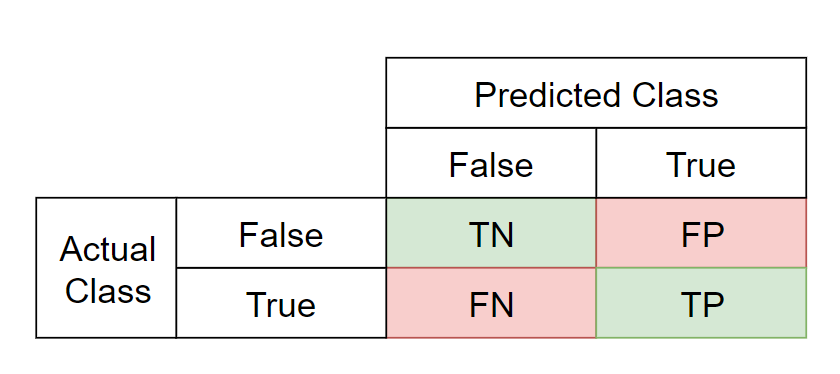
\includegraphics[scale = 0.3]{Images/2dconfusion.png}
  \caption{Confusion matrix for 2 classes.}
  \label{2classmatrix}
\end{figure}

Therefore, the most common metrics are: 

\begin{itemize}
  \item \textbf{Accuracy} (what \% of predictions were correct): $$ \cfrac{\text{number of corect predictions}}{\text{total number of predictions made}} = \cfrac{TP + TN}{TP + TN + FP + FN}$$ 
        Probably the most straightforward and intuitive metric for classifier performance. It is misleading when confronted with class imbalance problem, but for this project it is not the case. Hence, accuracy is an appropriate measure to estimate the performance of the models. 

  \item \textbf{Precision} (what \% of positive predictions were correct): $$ \cfrac{TP}{TP + FP}$$
        In the context of fraud detection, it is usually more costly to miss a positive instance than to falsely label a negative instance. Hence, we are concerned with precision rather than recall. 

  \item \textbf{Recall} (what \% of positive cases did model catch): $$ \cfrac{TP}{TP + FN}$$ 
        In situations where you want to detect instances of a minority class, one is usually concerned more with recall than precision. As stated in the Introduction, files' non-descriptive names might come as a result of intentional, adversarial, interaction with the file system, hence the interest in a great recall score.\\

  \item \textbf{F1 score} (weighted average of precision and recall): $$ \cfrac{2(\text{precision} \ * \ \text{recall})}{\text{precision} \ + \ \text{recall}} = \cfrac{2TP}{2TP + FP + FN}$$ 
        As all of the metrics above, F1 score takes values between 0 and 1, higher values indicating better performance. In fact, higher values of F1 score indicate better balance between precision and recall. 

  \item \textbf{Matthew's Correlation Coefficient (MCC)} $$ \cfrac{TP * TN - FP * FN}{\sqrt{(TP + FP)(TP + FN)(TN + FP)(TN + FN)}}$$ 
        Unlike the other metrics discussed above, MCC takes all the cells of the Confusion Matrix into consideration in its formula, hence behaves the best in case of imbalanced classes. The range of values of MCC lie between -1 to +1. A model with a score of +1 is a perfect model and -1 is a poor model, while a score of 0 is a as good as a random model. Although not facing the class imbalance problem, MCC would still make an excellent estimator for the overall performance of the ML models.
\end{itemize}

\subsubsection*{Metrics for MultiClass Classification}

In order to extend the 2D confusion matrix for the general case, I will adopt a One-vs-All (OVA) classifiers approach which reduces the problem to binary classification. Specifically, each class will be in turn considered the positive/true class, while all the others merged will be the negative/false class. At each step, the metrics described in the previous subsection will be computed and afterwards combined in a couple of different ways to form their variations used for evaluating multiclass classification. 

\begin{figure}[H]
  \centering
  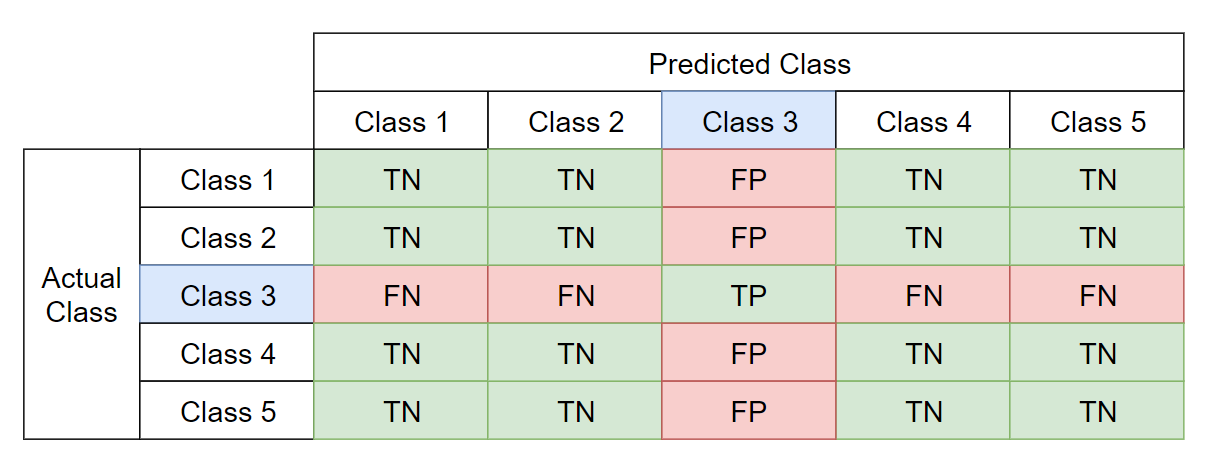
\includegraphics[scale = 0.4]{Images/5dconfusion.png}
  \caption{Confusion matrix for multiple classes using OVA approach where Class 3 is the positive class.}
  \label{5classmatrix}
\end{figure}

Let TP$_i$, TN$_i$, FP$_i$, FN$_i$ be the number of true positives, true negatives, false positives and false negatives when class $i$ is regarded as the positive class. Moreover, let Metric$_i$ be the value of an evaluation metric when class $i$ is regarded as the positive class, where Metric is one of Precision, Recall, F1 score, MCC (note that Accuracy will still be computed as before i.e. $ \frac{\text{number of corect predictions}}{\text{total number of predictions made}}$). Thus, Metric$_i$ is computed using TP$_i$, TN$_i$, FP$_i$, FN$_i$ as inputs. Given these definitions, there are two approaches to average the class specific metrics in order to obtain the metrics used for evaluating multiclass classifiers: 

\begin{itemize}
  \item \textbf{Micro Averaging}: \\
        Micro-Multiclass-Metric = Metric($\sum_{i=1}^{N}$ TP$_i$, $\sum_{i=1}^{N}$ TN$_i$, $\sum_{i=1}^{N}$ FP$_i$, $\sum_{i=1}^{N}$ FN$_i$) \\
        A micro-average will aggregate the contributions of all classes to compute the average metric. In a multi-class classification setup, micro-average is preferable when we suspect there might be class imbalance.

  \item \textbf{Macro Averaging}: \\
        Macro-Multiclass-Metric = $\tfrac{1}{N}$ $\sum_{i=1}^{N}$ Metric$_i$ \\
        A macro-average will compute the metric independently for each class and then take the average (hence treating all classes equally).
\end{itemize}

The evaluation will be conducted on balanced datasets, hence there is little difference expected between micro and macro averaging results and in the upcoming sections, I will report only in terms of macro averaging. 


\subsection{Monte Carlo Permutation Test}

In order to comparatively evaluate any two models implemented, I use the \textbf{permutation} \textbf{test}$^{\small \cite{permutation_test}}$ for paired samples. The permutation test checks whether the population mean of the two conditions is different (H$_1$) or the same (H$_0$). The power of the permutation test is defined as 1 - $\alpha$ where:

\begin{equation}
  \centering
  \alpha = \mathbb{P}(\text{Do not reject H$^0$ | H$_1$ is true} = \mathbb{P}(\text{test fails to detect the difference}) \newline
\end{equation}

I opted for the permutation test as it is known to have higher significance power than the, perhaps more popular, sign test$^{\small \cite{signtest}}$. The core assumption of the permutation test is that if the measured difference \textit{d} in mean M between systems A and B is an incident, i.e., if there is no real difference between them (because they come from one and the same distribution), it should not matter how many times one randomly swaps the two results. Consider \textit{n} paired results of System A and B. There are 2$^n$ ways of flipping or not flipping the n pairs of results, i.e., 2$^n$ permutations. These permutations operate row-wise. In other words, we create resamplings of these permutations in the following way: for each paired observation in the original runs, $a_i$ and $b_i$, a coin is flipped. If it comes up heads, then swap the score for $b_i$ with $a_i$. Otherwise, leave the pair unchanged. Now calculate the means M of the two system under this permutation, calculate their difference in means, and then do it 2$^n$ times for all permutations. Count how many of the 2$^n$ differences are as high as the difference in the unpermuted version. Call this number S. \smallskip

Finally, if due to a high number \textit{n}, the exponentially many resamplings computation is not feasible, then a large enough random subset of cardinality R should be tested. This version of the test is called \textbf{Monte Carlo Permutation Test}. The probability of observing the difference between the original runs by chance is approximated by: 

\begin{equation}
  p = \cfrac{S + 1}{R + 1}
\end{equation}

\smallskip

I decide that two sets of predictions come from different distributions for p-value $\leq$ 0.01 and I choose R = 5000.

\section{Evaluation Results and Discussions} \label{Evaluation Results}

The synthetic graphs for the first experiment conducted were generated using node properties and node degree distributions extracted from the real dataset. The experiment aimed to determine how the Patchy-San CNN pipeline performs depending on the Interaction Depth (ID) and History Depth (HD) parameters of the synthetic graphs. The NN used in this case was not tuned in any way, hyperparamer values being picked from popular choices in the research field. Figure \ref{inter_hist_depth_acc} highlights that cases in which: 
(a) only processes that directly interact with multiple versions of a file are considered(i.e. ID = 1) or (b) only processes that interact with a single version of a file, in one or multiple hops are considered (i.e. HD = 1). In both scenarios the dimensions of the provenance subgraphs for each node increases considerably before the NN can overcome the 0.9 accuracy threshold. In contrast, using both history and interaction dimensions achieves perfect accuracy much easier, for instance, on graphs where ID = 3 and HD = 4. Therefore, using both higher order ancestors and past information is of paramount importance when selecting the provenance graph for a specific file. 


\begin{figure}[H]
  \centering
  \centerline{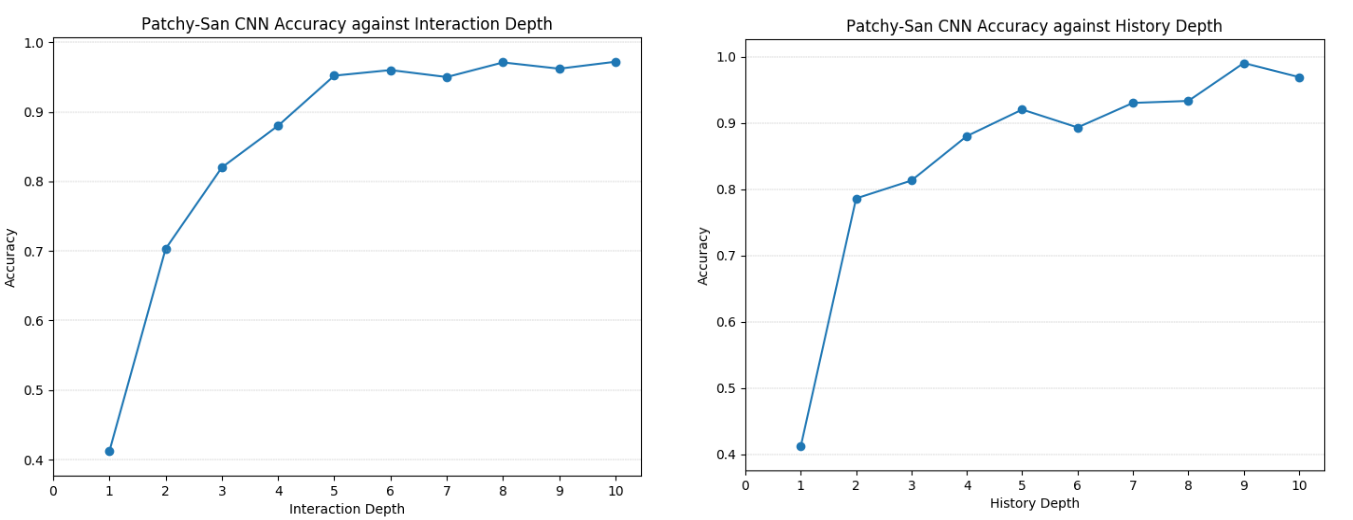
\includegraphics[scale=0.475]{Images/inter_hist_deph_acc.png}}
  \caption{ Figure showing accuracy scores for various values of $ID$ keeping $HD = 1$ (LHS) and
    accuracy for various values of $HD$ keeping $ID = 1$ (RHS).}
  \label{inter_hist_depth_acc}
\end{figure}

The perfect accuracy previously obtained for Patchy-San CNN is easily replicated by both baseline models. This comes from the fact that the real dataset lacks in richness and the node properties distributions extracted are easily distinguishable. To characterise these distributions better I take into account their L2$_{\text{distance}}$ from the uniform distribution, which is defined in Equation \ref{l2_distance}.  

\begin{equation} 
    \centering
    \text{L2}_\text{distance}\text{(p)} = \sqrt{\sum_{i=1}^{n} (p_i - \tfrac{1}{n})^2} \in [0,\sqrt{2}] \newline
\end{equation} \label{l2_distance}

$$ \text{where p = }(p_1, p_2, ..., p_n) \ \text{is a probability distribution.} $$ 

I say that a set of distributions are in range [0, K] when the greatest L2$_{\text{distance}}$ among them is less or equal to K. Real graph distributions are in range [0, 0.45]. The following experiment, illustrated in Figure \ref{l2_dist}, aims to test how the Patchy-San CNN pipeline behaves when dealing with node properties distributions closer to uniform than those in the real dataset. This would implicitly make the distributions closer to each other and not as easily distinguishable by the ML model. 

\begin{figure}[H]
  \centering
  \centerline{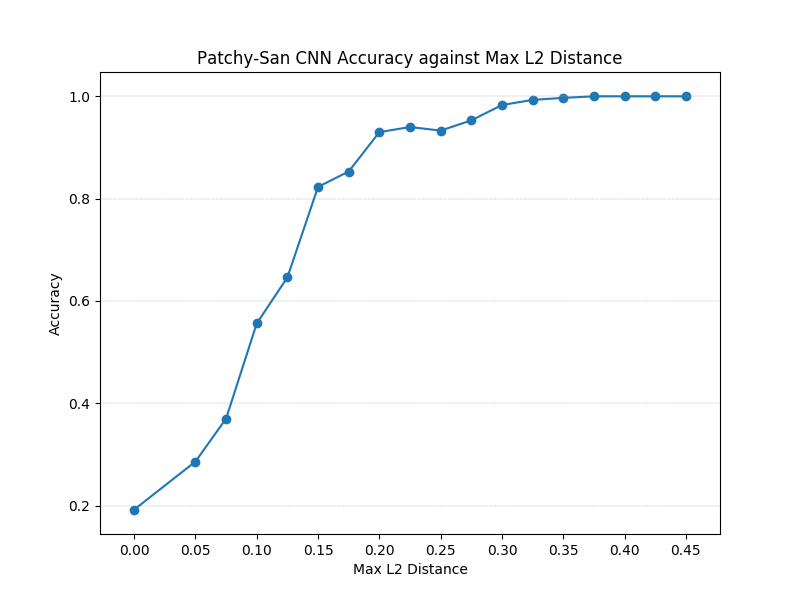
\includegraphics[scale=0.3]{Images/l2_dist.png}}
  \caption{ Figure showing accuracy scores for various values of maximum $\text{L2}_{\text{distance}}$ for $ID = 3$ and $HD = 4$.}
  \label{l2_dist}
\end{figure}

Given the results of the first two experiments, all of the following evaluations were conducted on 3000 log files and 3000 synthetic graphs with ID = 3 and HD = 4, uniformly split into 6 classes. Node probability distributions were in range [0, 0.2] (way more restrictive than in the real dataset). \smallskip

By obtaining the highest metrics in each section, as shown in Table 4.1, CNN outperforms Random Forest and KNN in the graph classification task, on this specific dataset. These results were expected, as all the complex preprocessing executed by the Patchy-San algorithm was meant to exploit structural properties of the graphs (aspect that none of the baseline models takes into account). However, given the outcomes of the permutation test (Table \ref{p_values}), there is a statistically significant difference only between CNN and KNN, whereas between CNN and Random Forest the probability that the results were obtained by chance is above the 0.01 established threshold, hence the Null Hypothesis cannot be rejected. 

%\begin{longtable}{|p{.185\textwidth}|p{.15\textwidth}|p{.15\textwidth}|p{.15\textwidth}|p{.15\textwidth}|p{.15\textwidth}|}
 % \hline
 %                    & \textbf{K-nearest Neighbours} & \textbf{Randon Forest}        & \textbf{CNN}        & \textbf{MLP} & \textbf{Stacking Ensemble}                                      \\
 % \hline
  %\textit{Accuracy}  & $0.786 \pm 0.040 $          & $0.873 \pm 0.026 $ &\cellcolor{green!50} $0.928 \pm 0.012 $ &   $0.911 \pm 0.018 $  & $0.900 \pm 0.010 $ \\
 % \hline

  %\textit{Macro Precision}   & $0.790 \pm 0.037 $          & $0.877 \pm 0.022 $ & \cellcolor{green!50} $0.925 \pm 0.014 $ &   $0.913 \pm 0.017 $  & $0.901 \pm 0.014 $ \\
  %\hline

  %\textit{Macro Recall}       & $0.823 \pm 0.026 $          & $0.866 \pm 0.021 $ & \cellcolor{green!50} $0.927 \pm 0.011 $ &   $0.909 \pm 0.020 $  & $0.905 \pm 0.013 $ \\
  %\hline

  %\textit{Macro F1 Score}      & $0.785 \pm 0.041 $          & $0.876 \pm 0.024 $ &\cellcolor{green!50} $0.924 \pm 0.013 $ &   $0.912 \pm 0.180 $  & $0.901 \pm 0.015 $ \\
  %\hline

   %\textit{Macro MCC}      & $0.754 \pm 0.041 $          & $0.850 \pm 0.025 $ &\cellcolor{green!50} $0.913 \pm 0.015 $ &   $0.898 \pm 0.150 $  & $0.883 \pm 0.017 $ \\
 % \hline
  %\caption{Evaluation results for the models implemented.}
 % \label{results}
%\end{longtable}

\begin{figure}
    \centering
    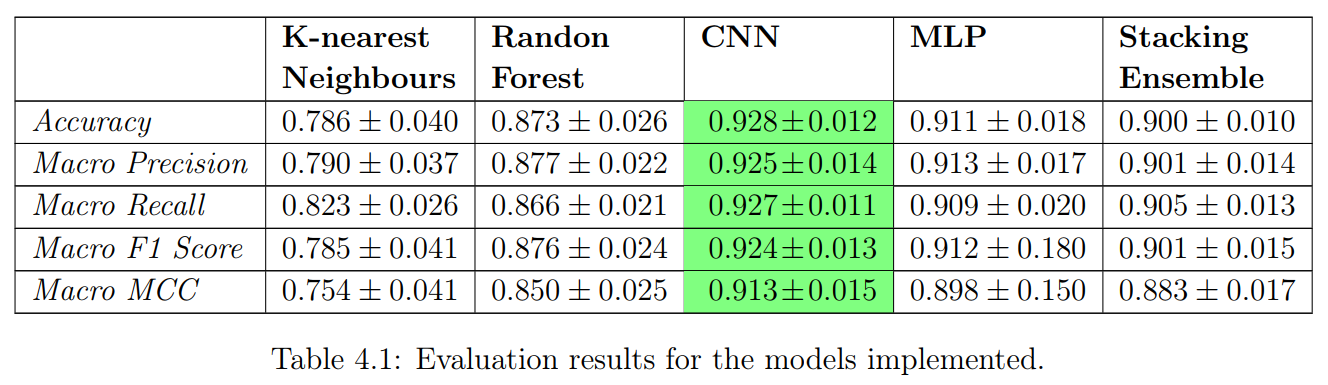
\includegraphics[scale = 0.335]{Images/results_table.png}
    \label{results}
\end{figure}

The second highest metrics in each sections were achieved by the MLP. This reveals that the content classification module was also a success, having great balance between precision and recall. The intriguing results are those of the permutation test, which suggest that MLP is statistically significantly different from all the other models. This means that the model outperforms KNN, RF and the stacked ensemble, while being outperformed by CNN. The fact that MLP is trained and tested on differently structured information should not matter for this result, as p-values are only computed w.r.t. the output labels. One case in which MLP does show slightly undesirable results can be observed in Figure \ref{mlp_train_test}. On every outer fold of the NCV, when training the MLP, it rapidly converges to perfect accuracy. Contrary, while testing the MLP, although it achieves great accuracy scores just as fast as when training, there is some variation as epochs are passing. Specifically, the accuracy oscillates up and down, roughly in a 0.1 range. These might suggest that, despite the regularisation techniques applied, some of the hyperparameters were overfitted on the training set.

\begin{figure}[H]
  \centering
  \centerline{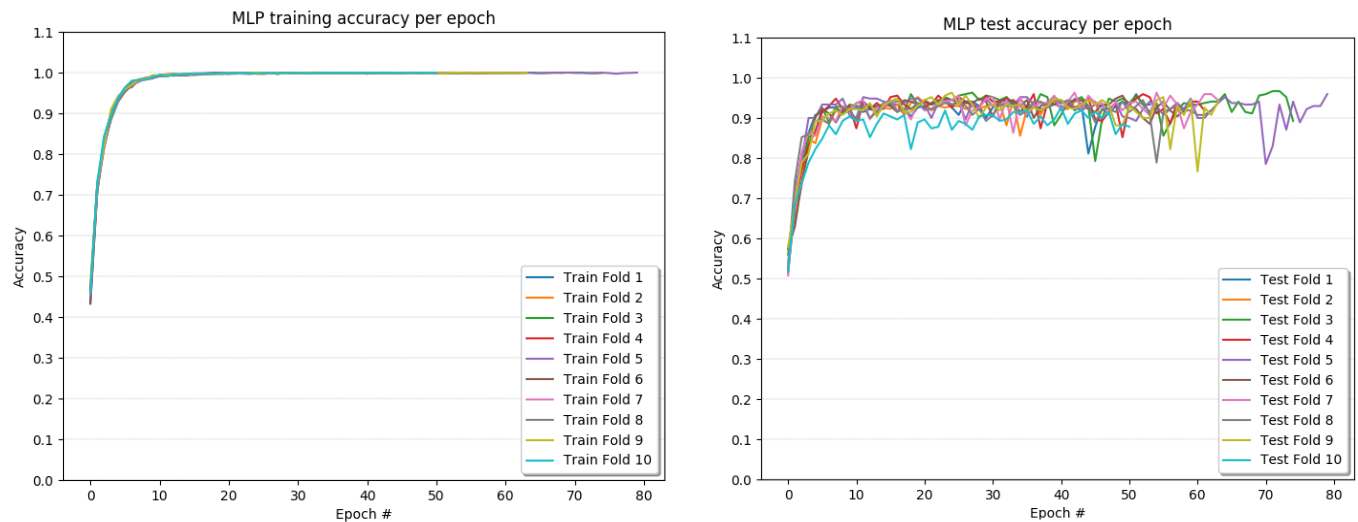
\includegraphics[scale=0.475]{Images/mlp_train_test.png}}
  \caption{MLP training and test accuracy against training epoch.}
  \label{mlp_train_test}
\end{figure}

KNN achieves the lowest results on every analysed metric. Moreover, the permutation test confirms that there is also statistical different between KNN and all other models, classifying it as the worst performing algorithm. Another aspect in which KNN behaves poorly is the variance across the scores between the 10 outer folds of the NCV, as depicted in Figure \ref{acc_per_fold} and Figure \ref{macro_mcc_per_fold}. 

\begin{figure}[H]
  \centering
  \centerline{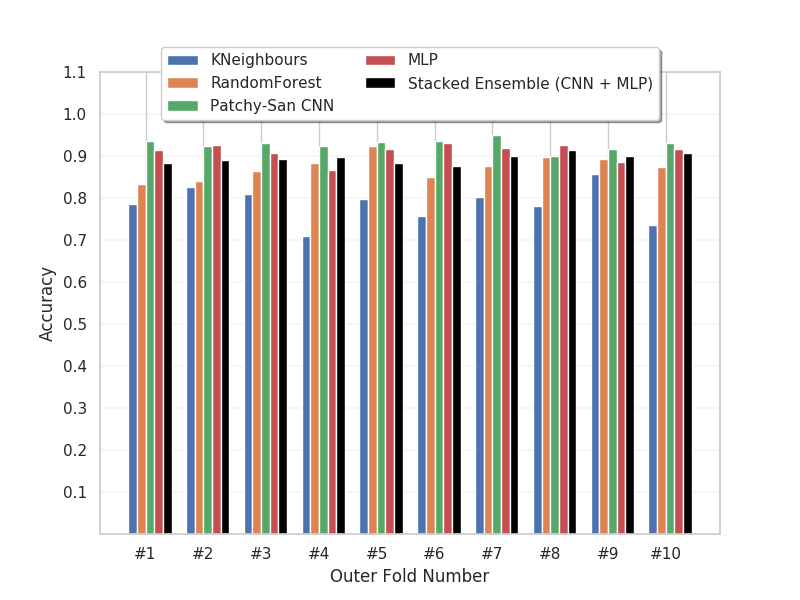
\includegraphics[scale=0.58]{Images/acc_per_fold_new_cols.png}}
  \caption{Comparative accuracy scores for all implemented models per outer fold.}
  \label{acc_per_fold}
\end{figure}

\begin{figure}[H]
  \centering
  \centerline{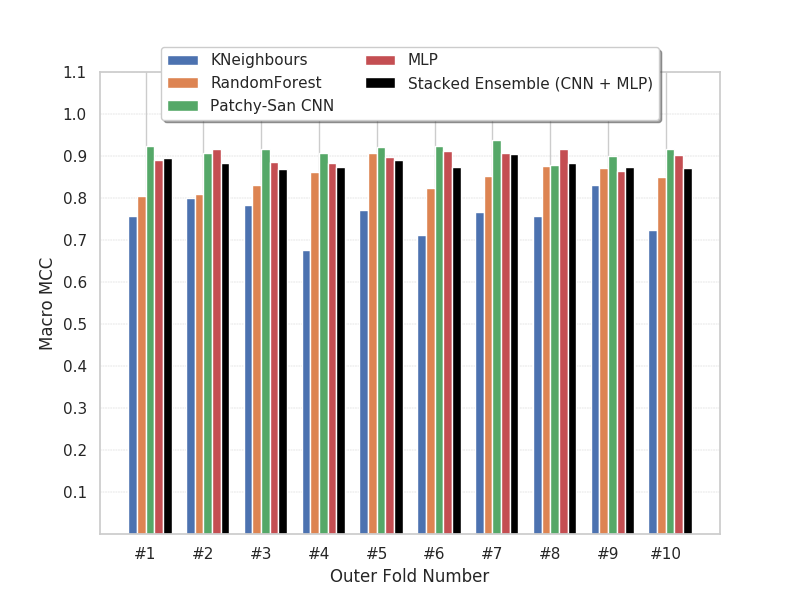
\includegraphics[scale=0.58]{Images/macro_mcc_per_fold_new_cols.png}}
  \caption{Comparative macro MCC scores for all implemented models per outer fold.}
  \label{macro_mcc_per_fold}
\end{figure}

On the opposite side, CNN not only presents the less variation across the splits for both accuracy and macro MCC, but it also achieves the highest metrics in 8 out of 10 scenarios. Furthermore, Figure \ref{cnn_train_test} shows that on each test fold, CNN follows a steep path, rapidly converging (w.r.t. the number of epochs needed - about 10 to 15) to the achieved results, point where it saturates and the variations are minimal. In fact, the high resemblance between the training and testing curves on all folds, is yet another proof that the model generalises well and there is no sign of overfitting. 

\begin{figure}[H]
  \centering
  \centerline{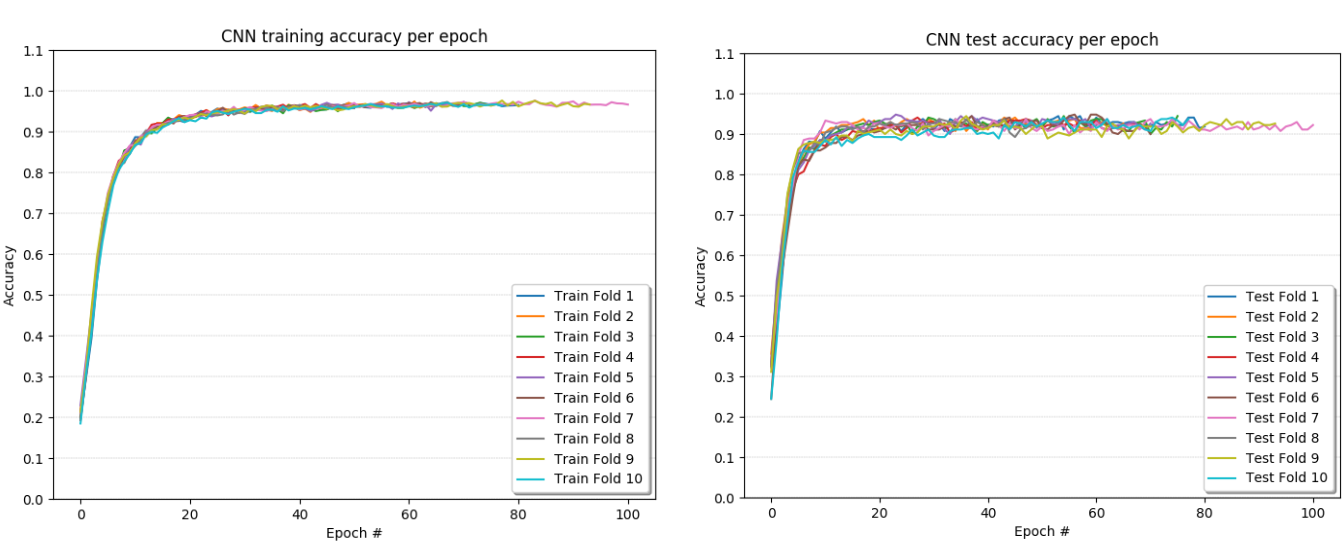
\includegraphics[scale=0.475]{Images/cnn_train_test.png}}
  \caption{CNN training and test accuracy against training epoch.}
  \label{cnn_train_test}
\end{figure}

Usually, ML ensembles are constructed to combine the predictions of multiple weaker classifiers and improve the overall results. On the chosen dataset, not only does it achieve worse results than both of the base classifiers that it is comprised of, but the permutation test also suggest that there is statistical difference between the ensemble and MLP. This happens due to two main considerations. Firstly, the ensemble was obtained by combining the greatest predictions (w.r.t. accuracy score) of MLP and CNN across the entire NCV procedure. This approach does not take into account the situation in which base learners with worse individual scores might actually result in the best overall model. Secondly, such an ensemble might have required more that just a couple of learners to actually present any improvement. Nonetheless, this model is still extremely capable, successfully combining context and content information, thus accomplishing one of the project's success criteria. \\

In conclusion, 4 out of 5 implemented models are extremely competent in this classification task, achieving great results on the synthetically created dataset. Patchy-San CNN pipeline is the best all around model, which generalises well and hence successfully harvests graphs structural properties. 

\begin{figure}[H]
  \centering
  \centerline{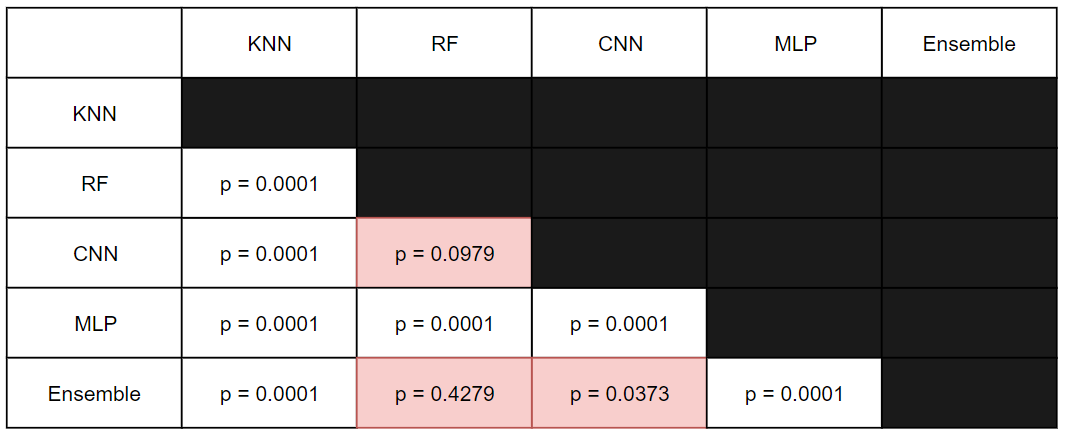
\includegraphics[scale=0.43]{Images/p_values.png}}
  \caption{Permutation test pairwise results. Highlighted in red are values over the 0.01 established threshold.}
  \label{p_values}
\end{figure}


\end{document}


